\documentclass[a4paper,11pt]{article}

%A Few Useful Packages
\usepackage{marvosym}
\usepackage{fontspec} 					%for loading fonts
\usepackage{xunicode,xltxtra,url,parskip} 	%other packages for formatting
\RequirePackage{color,graphicx}
\usepackage[usenames,dvipsnames]{xcolor}
\usepackage[big]{layaureo} 				%better formatting of the A4 page
% an alternative to Layaureo can be ** \usepackage{fullpage} **
\usepackage{supertabular} 				%for Grades
\usepackage{titlesec}					%custom \section
\usepackage{xeCJK}						%chinese
\usepackage{graphicx}
\usepackage{geometry}
\usepackage{wrapfig}
\usepackage{multirow}

%\geometry{papersize={20cm,15cm}}
\geometry{top=1cm,bottom=1cm}


%Setup hyperref package, and colours for links
\usepackage{hyperref}
\definecolor{linkcolour}{rgb}{0,0.2,0.6}
\hypersetup{colorlinks,breaklinks,urlcolor=linkcolour, linkcolor=linkcolour}

%FONTS
\defaultfontfeatures{Mapping=tex-text}
%\setmainfont[SmallCapsFont = Fontin SmallCaps]{Fontin}
\setmainfont[BoldFont={Hei}]{STXihei}
%%% modified for Karol Kozioł for ShareLaTeX use
%\setmainfont[
%SmallCapsFont = Fontin-SmallCaps.otf,
%BoldFont = Fontin-Bold.otf,
%ItalicFont = Fontin-Italic.otf
%]
%{Fontin.otf}
\setCJKmainfont[BoldFont={Hei}]{STXihei} %设置 CJK 主字体为 SimSun (宋体)

%%%

%CV Sections inspired by:
%http://stefano.italians.nl/archives/26
\titleformat{\section}{\Large\scshape\raggedright}{}{0em}{}[\titlerule]
\titlespacing{\section}{0pt}{3pt}{3pt}
%Tweak a bit the top margin
%\addtolength{\voffset}{-1.3cm}

%Italian hyphenation for the word: ''corporations''
\hyphenation{im-pre-se}

%-------------WATERMARK TEST [**not part of a CV**]---------------
\usepackage[absolute]{textpos}

\setlength{\TPHorizModule}{30mm}
\setlength{\TPVertModule}{\TPHorizModule}
\textblockorigin{2mm}{0.65\paperheight}
\setlength{\parindent}{0pt}

%--------------------BEGIN DOCUMENT----------------------
\begin{document}

%WATERMARK TEST [**not part of a CV**]---------------
%\font\wm=''Baskerville:color=787878'' at 8pt
%\font\wmweb=''Baskerville:color=FF1493'' at 8pt
%{\wm
%	\begin{textblock}{1}(0,0)
%		\rotatebox{-90}{\parbox{500mm}{
%			Typeset by Alessandro Plasmati with \XeTeX\  \today\ for
%			{\wmweb \href{http://www.aleplasmati.comuv.com}{aleplasmati.comuv.com}}
%		}
%	}
%	\end{textblock}
%}

\pagestyle{empty} % non-numbered pages

\font\fb=''[cmr10]'' %for use with \LaTeX command

%--------------------TITLE-------------
\par{
		\begin{center}{\Huge 李雪楠
	}\end{center}

\par}

%--------------------SECTIONS-----------------------------------
%Section: Personal Data
\section{基本信息}

\begin{tabular}{rlrr}
  &生日: 1994.11.15 & \quad\quad\quad\quad\quad\quad\quad\quad & \multirow{6}{*}{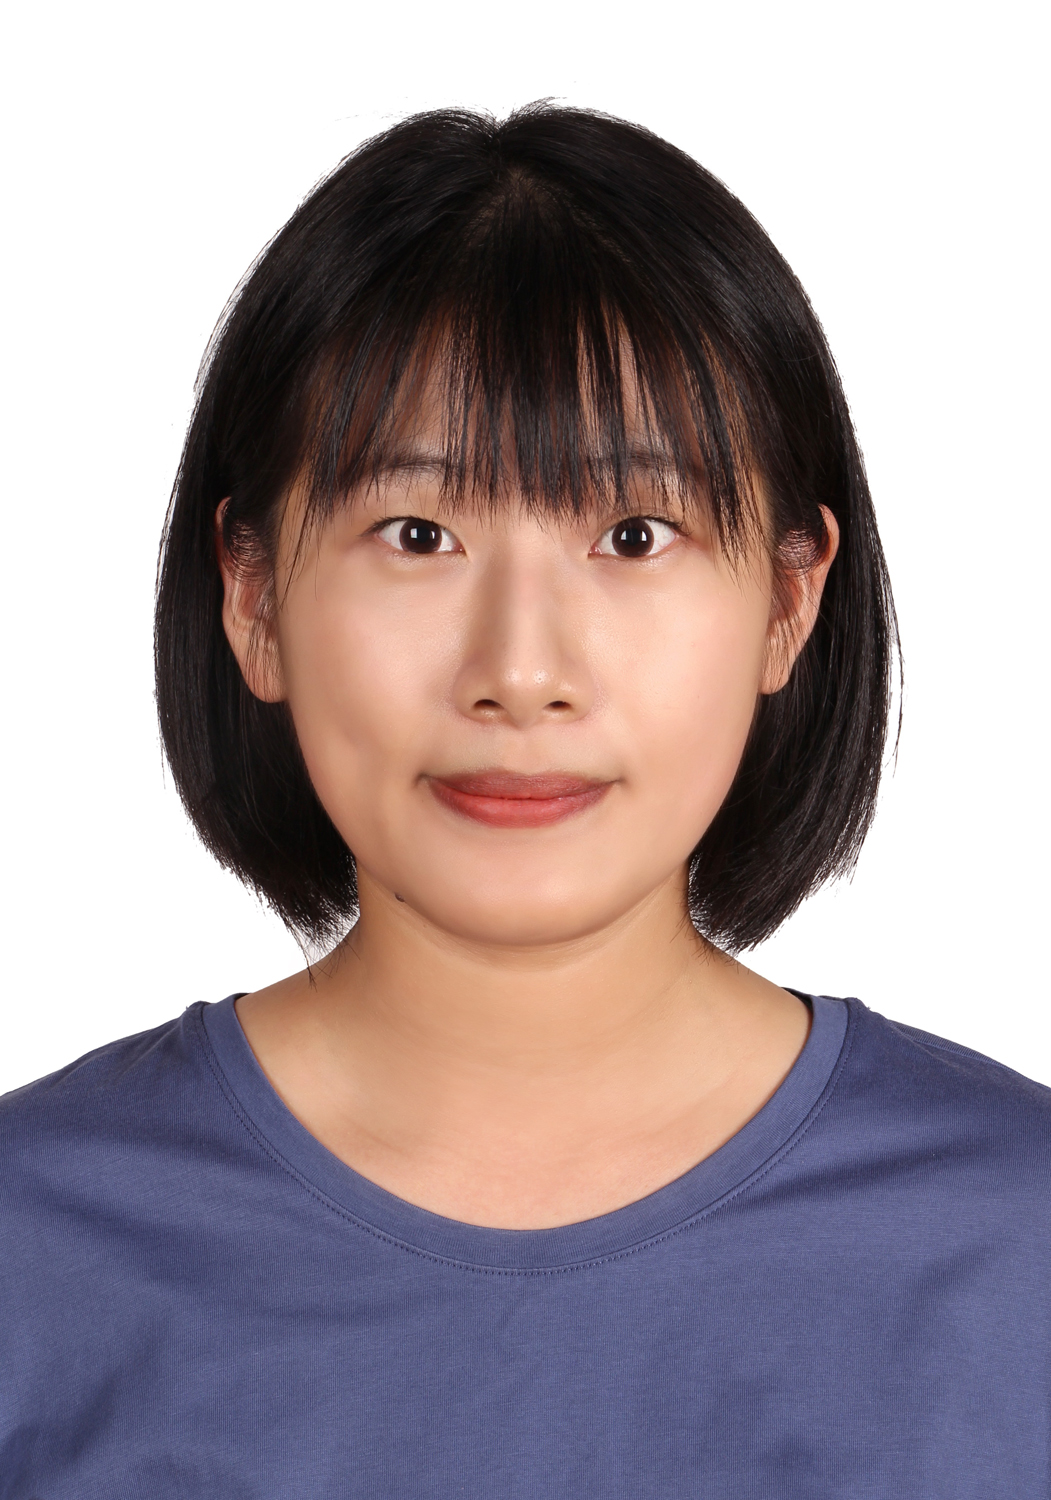
\includegraphics[width=0.18  \textwidth]{baby.jpg}}\\
  &籍贯: 河南汤阴 \\
  &地址: 浙江省杭州市浙江财经大学下沙校区\\
  &手机: 13512104561\\
  &邮箱: \href{mailto:1755340412@qq.com}{1755340412@qq.com}\\
  &政治面貌: 中共党员\\
  \\
\end{tabular}



%Section: Education
\section{学习经历}
\begin{tabular}{rl}
\textsc{2012.9-2016.7} & 本科, 山西财经大学, 公共管理学院, 人力资源管理专业\\
& 主修课程: 绩效管理, 薪酬与福利管理,组织行为学\\&\\
\textsc{2018.9-2021.3} & 硕士研究生, 浙江财经大学, 马克思主义学院, 伦理学专业\\
& 主修课程: 经济伦理学, 道德心理学, 中国特色社会主义理论与实践研究\\&\\
\end{tabular}


%Section: Work Experience at the top
\section{工作经历}
\begin{tabular}{r|p{11cm}}
 \textsc{2017.4-8} & 中青旅集团上海控股有限公司, 人事助理 \\&负责档案的整理和电子档案信息的录入;部门日常采购;微信公众号的撰写以及领导安排的其他工作。\\\multicolumn{2}{c}{} \\
\end{tabular}

%Section: Work Experience at the top
\section{课题研究}
\begin{tabular}{r|p{11cm}}
\textsc{2020.11} & 哈耶克自由主义经济伦理思想研究\\&本课题涉及哲学、经济学、法学、伦理学等多学科,结合中国改革开放以来所取得的经济成就,指出个体在此形势下取得的所做出的贡献,阐述了哈耶克经济伦理思想的主要内容;结合新冠疫情,对哈耶克自由理念以及他对经济体制所做出的道德判断来进行批判,并通过中国在应对疫情时所做出的举措,来指出社会主义制度的优越性。\\\multicolumn{2}{c}{} \\
\end{tabular}

%Section: Work Experience at the top
\section{社会实践}
\begin{tabular}{r|p{11cm}}
\textsc{2019-2020} & 多次参加浙江财经大学图书馆志愿活动\\&帮助老师整理相关书籍和期刊的摆放,帮助老师和同学第一时间获取新的书籍。\\\multicolumn{2}{c}{} \\
\end{tabular}

%Section: Scholarships and additional info
\section{获奖经历\&证书}
\begin{tabular}{rl}
 \textsc{2018}  & 浙江财经大学研究生团队合作英语口语报告竞赛三等奖\\
 \textsc{2019} & 浙江财经大学研究生科研论文报告会优秀奖\\

\end{tabular}

%Section: Languages
\section{语言能力}
\begin{tabular}{rl}
&英语: CET4\\
&普通话二级甲等\\
\end{tabular}

\section{专业技能}
\begin{tabular}{rl}
&计算机二级证书,熟练使用 Office 相关办公软件\\
\end{tabular}

\section{兴趣爱好}
\begin{tabular}{rl}
&游泳~~爬山~~音乐
\end{tabular}



\end{document}
